\documentclass{article}
\usepackage{graphicx}

\title{C# Reverse Engineering}


\begin{document}
\maketitle

\section*{C# compilation process}
C# --> CIL --> machine code

\begin{figure}
    \centering
    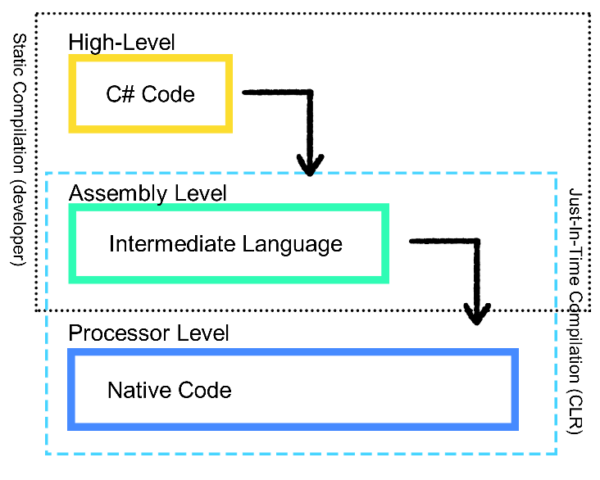
\includegraphics[width=10cm]{how-is-c-compiled_01-600x480.png}
    \caption{TBD}
    \label{fig:TBD}
    % https://freecontent.manning.com/how-is-c-compiled/
\end{figure}

\end{document}